% Historique du sujet
% Introduction théorique
% Application dans la vie courante

Le solénoïde est un dispositif beaucoup utilisé dans la vie quotidienne, grâce a ces caractéristiques d’électro-aimant. L’exemple le plus simple est le suivant: lorsqu'on insère la clé de contact dans une voiture, le signal du démarrage du moteur est transmit via un solénoïde. On peut le retrouver dans d'autres domaines comme la sécurité à fermeture magnétique, la médecine, l'automobile, dans les enceintes ou amplificateurs audio, etc.\\
Elle possède des propriétés électromagnétiques car associée à un aimant ou une autre bobine, elle peut servir de transformateur de tension, de mécanisme de moteur, d'interrupteur ou encore de microphones. Ce dispositif peut être couplés ou non avec d'autres composants.\\
Un solénoïde est plus précisément une bobine allongée constituée d'un fil conducteur enroulé. C'est pourquoi ce dernier peut aussi prendre le terme de bobine. Lorsqu'il est parcouru par un courant électrique, il va créer une force magnétique selon son axe d’enroulement.
\begin{figure}[H]
  \centering
    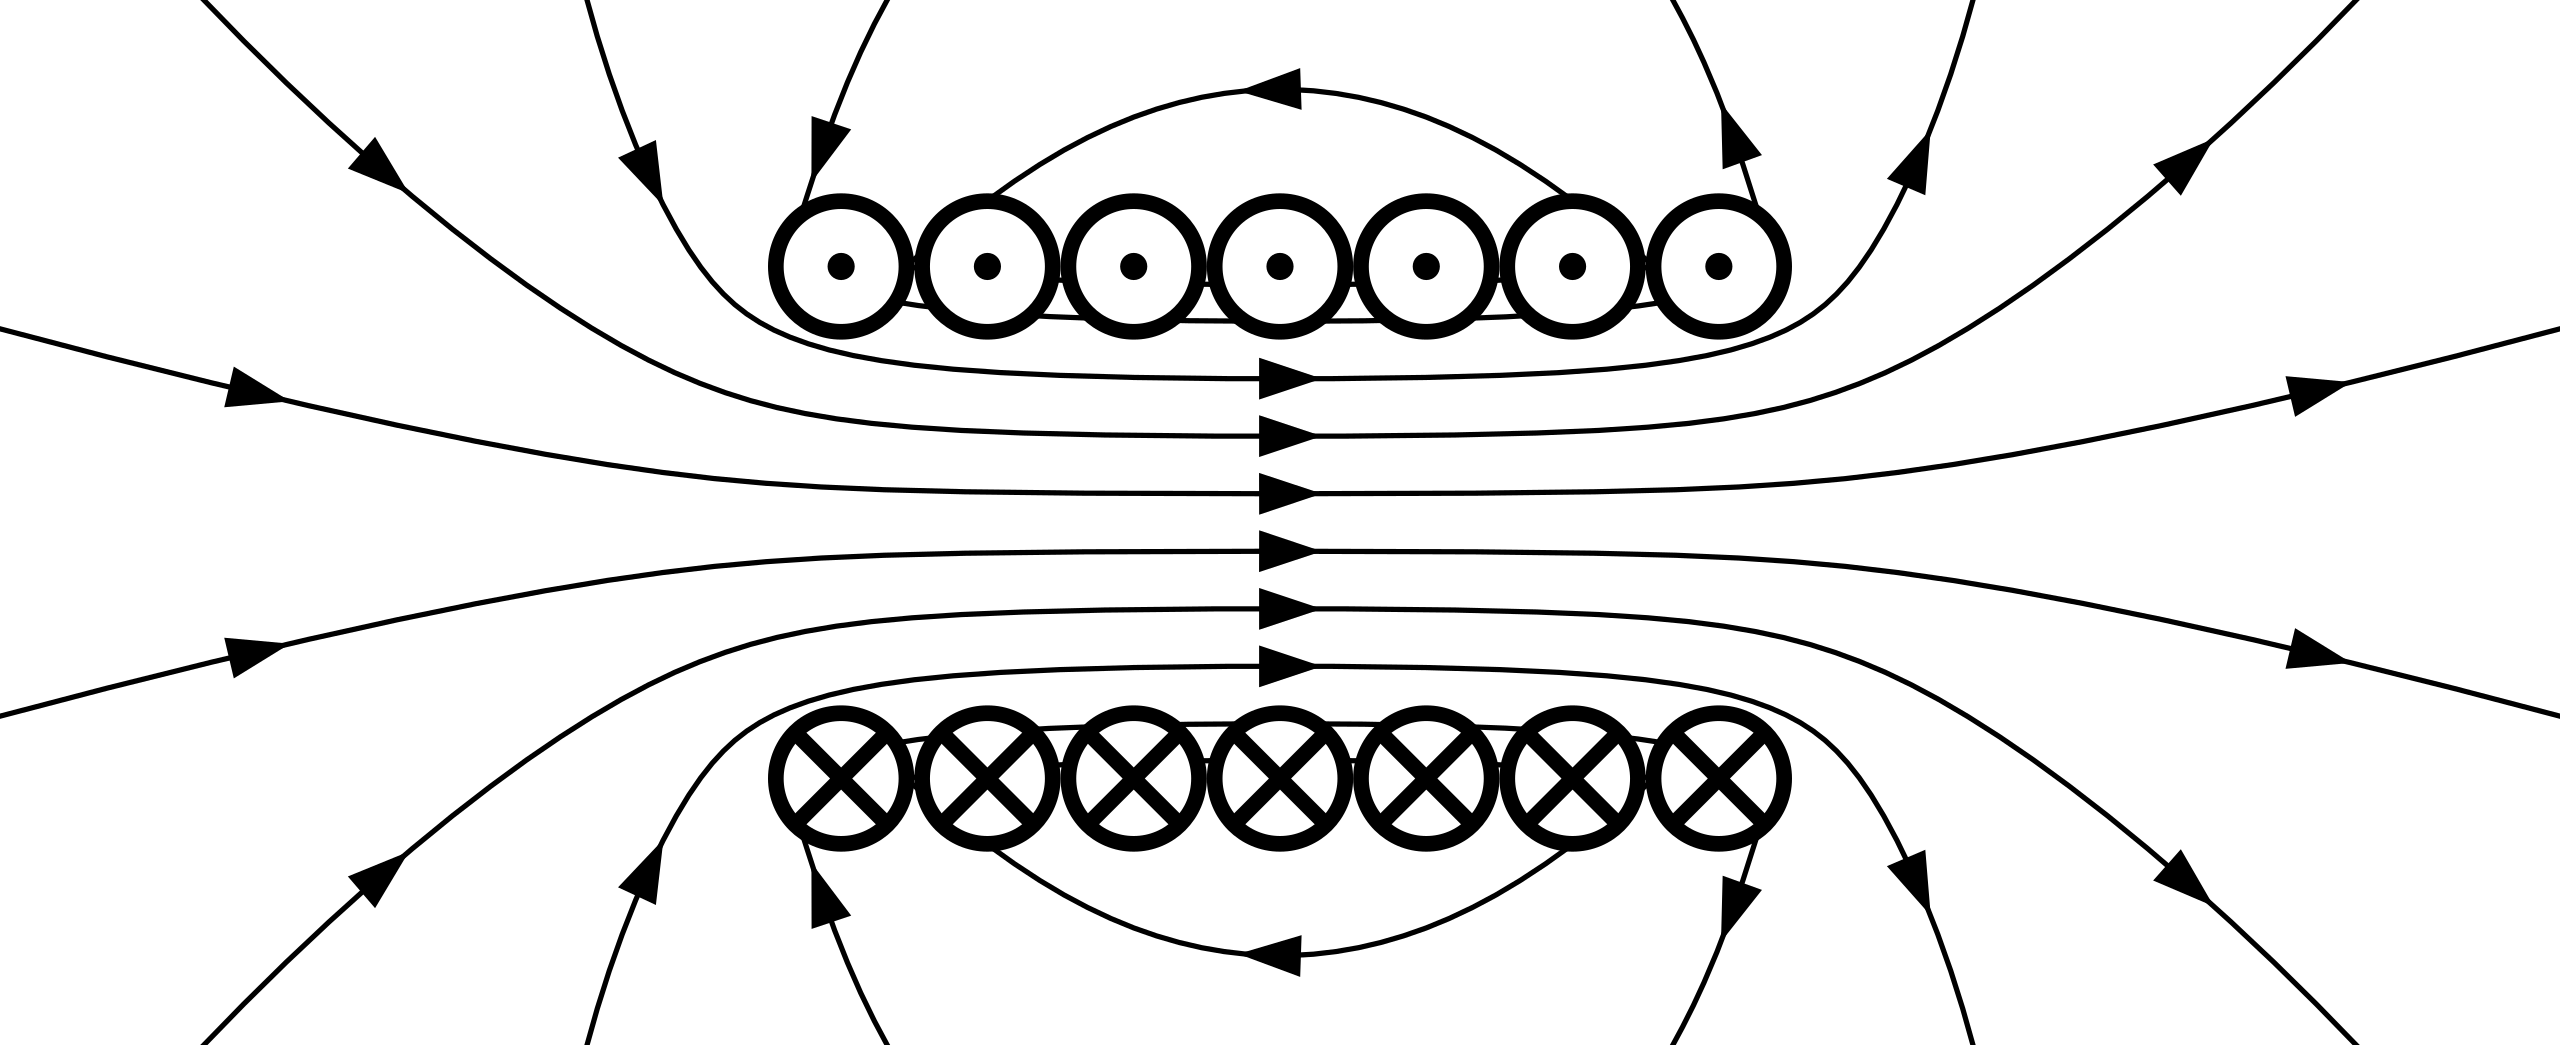
\includegraphics[width=0.3\textwidth]{Sol_champ.png}
    \caption{Image de \emph{Wikipedia} "Solénoïde"}
\end{figure}


C'est en 1831, que le scientifique britannique Michael Faraday étudie le comportement d'un courant dans un champ magnétique, et s'aperçoit que celui-ci peut produire du travail. Ørsted avait découvert qu'un courant électrique produit un champ magnétique. Suite à cela, Faraday découvre qu'un champ magnétique peut aussi engendrer un courant électrique. Il découvre ainsi le principe du moteur électrique, et donc la conversion du travail mécanique en énergie électrique, inventant ainsi le générateur de courant. Dans un article de 1852, Faraday dévoile l'existence du champ magnétique en décrivant les « lignes de force » le long desquelles s'oriente la limaille de fer au voisinage de l'aimant.\\

Un solénoïde idéal fait preuve de la propriété suivante : parcouru par un courant, le champs à l'intérieur est homogène, et nul à l'extérieur. Concrètement, ces conditions ne sont qu'atteignable si le solénoïde est de longueur infinie ou pouvant être approximé comme telle. Donc, en ne prenant qu'une portion du solénoïde et le considérant parfait, la loi d'Ampère peut être appliquée:
$$
    Bl = \mu_0 NI 
$$
avec $B$ le champs magnétique, $l$ la longueur, $\mu_0$ la perméabilité du vide (également nommée perméabilité magnétique du vide ou constante magnétique), $I$ l'intensité et $N$ le nombre de spires.\\
Sauf que l'idée d'un tube infini n'est pas réel. Cette formule sert d'une approximation de la réalité. En théorie, le comportement d'un solénoïde idéal diffère de la pratique.
\begin{figure}[H]
  \centering
  \begin{minipage}[b]{0.4\textwidth}
    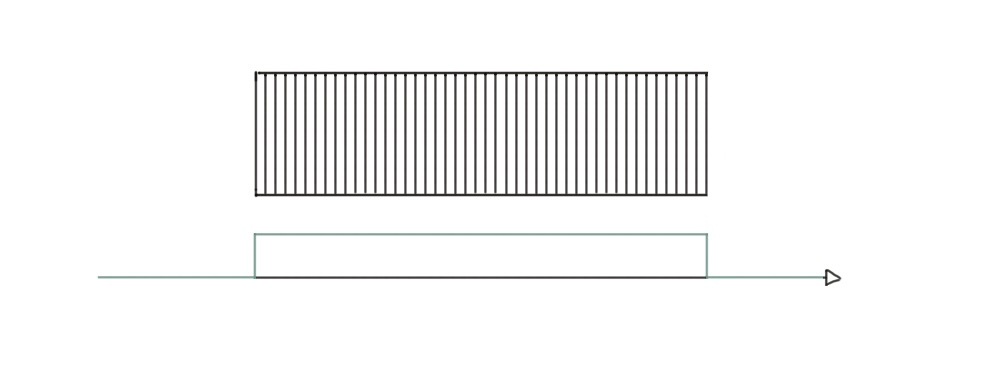
\includegraphics[width=\textwidth]{Sol_champ_id}
    \caption{Champs d'un solénoïde idéal}
  \end{minipage}
  \hfill
  \begin{minipage}[b]{0.4\textwidth}
    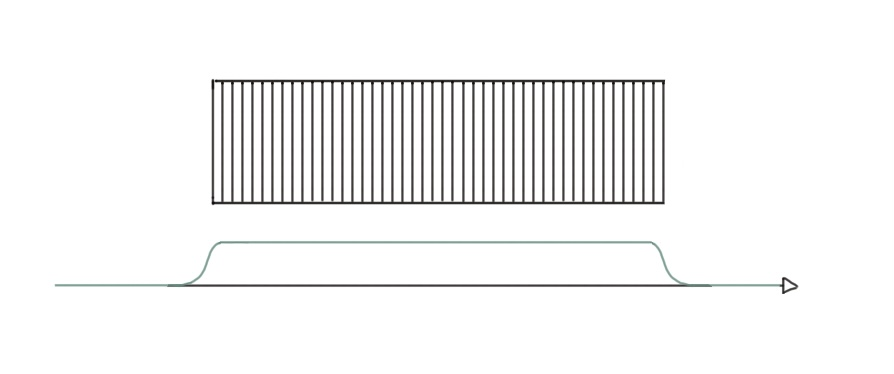
\includegraphics[width=\textwidth]{Sol_champ_re}
    \caption{Champs d'un solénoïde en pratique}
  \end{minipage}
\end{figure}
Sur l'axe est représentée la force du champ magnétique des solénoïde. En réalité, le champ ne se rompt pas d'un coup aux extrémités de la bobine. Par consequent, le champ n'est pas identique aux extrémités et au centre. En effet, la force du champs augmente progressivement avant de se stabiliser, puis diminue.\\

Considérons une bobine de longueur $l$, de rayon $R$, contenant $N$ spires et traversée par un courant $I$, où l'on cherche à trouver le champs $\vec{B}$ au point $P$. Ce dernier est déterminé par les angles $\theta_1$ et $\theta_2$.
\begin{figure}[H]
  \centering
    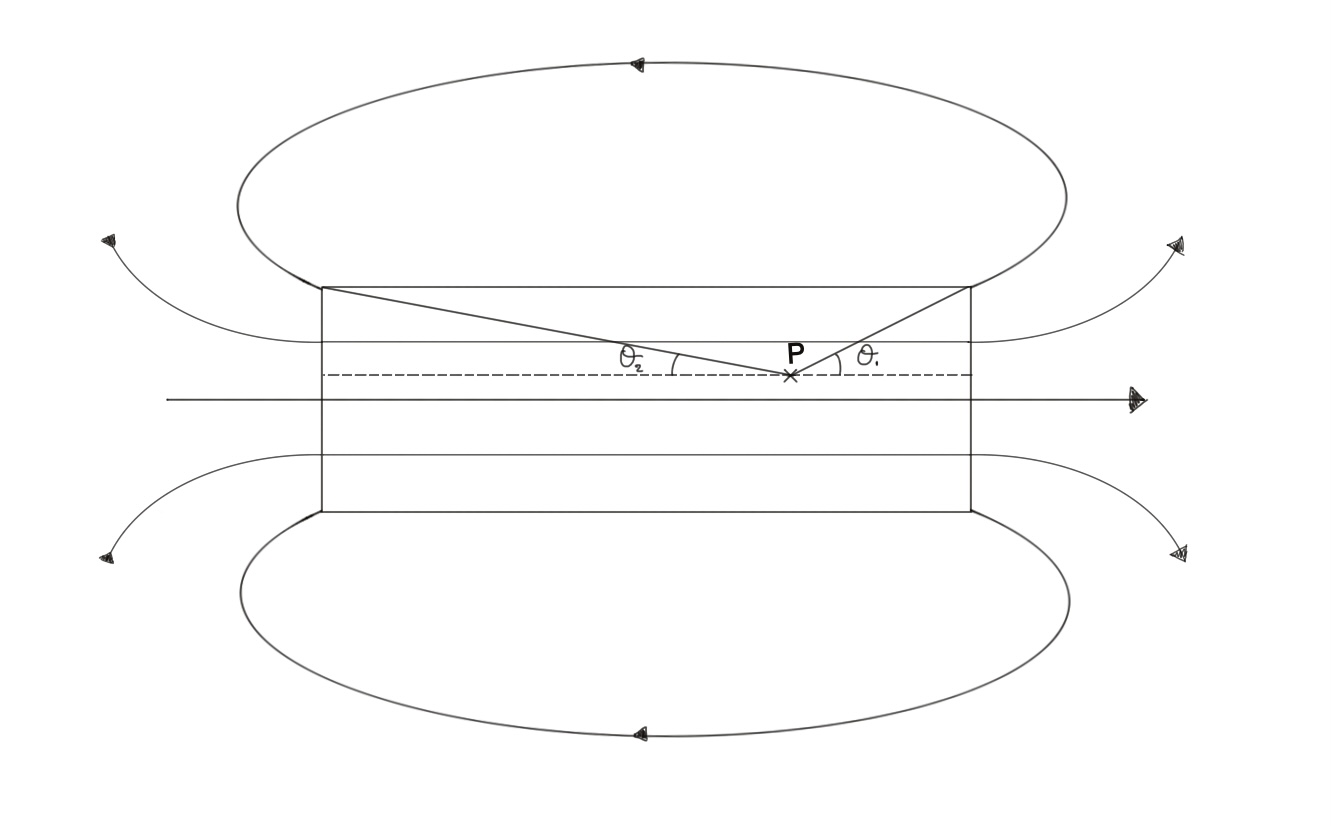
\includegraphics[width=0.5\textwidth]{Sol_P1}
\end{figure}

\begin{invsummary}
La relation est définie comme suit :
$$ B = \frac{N I \mu_0}{l} \frac{\cos \theta_1 + \cos \theta_2}{2} $$
et afin de la prouver, on doit commencer par regarder le champ magnétique généré par un cercle en un point $x$ au dessus de son centre.
\end{invsummary}

\begin{summary}
Sachant que le cercle de rayon $R$ peut se définir comme suit :
$$ \vec{l} = \begin{pmatrix}
R \cdot \sin t \\
R \cdot \cos t \\
0
\end{pmatrix} $$
et en utilisant la relation issue de la loi de Biot-Savart
$$\vec{B}(\vec{r}) = \frac{\mu_0}{4\pi}\int_t \frac{I \frac{d\vec{\ell}}{dt} \times (\vec{r}-\vec{\ell})}{|\vec{r}-\vec{\ell}|^3} dt $$
sur un point respectant la condition énoncée ci-dessus
$$ \vec{r} = \begin{pmatrix}
0\\
0\\
x
\end{pmatrix} $$
nous pouvons effectuer l'intégral via le module \emph{Python} nommé \emph{sympy}, ce qui nous donne le résultat\footnotemark
$$ B(x) = \frac{I R^2 \mu_0}{2 \left( x^2 + R^2 \right)^{\frac{3}{2}}} $$
\end{summary}

\begin{invsummary}
La suite est de considérer un solénoïde de $2N$ spires et de longueurs $2l$. Considérons le point $x$ sur l'axe centrale de ce solénoïde. Le champs magnétiques en ce point peut être approximé par la somme du champs créer par des cercle infinitésimaux sur toute la longueur du solénoïde, que l'on connaît par la formule ci-dessus. Sachant qu'il y a donc des portions de courant proportionnel à la longueur et au nombre de spire $dI = \frac{dt}{l}NI$ avec $dt$ une portion de distance. On peut ensuite poser l'intégrale :
$$ B(x) = \int \frac{dI R^2 \mu_0}{2 \left( (t-x)^2 + R^2 \right)^{\frac{3}{2}}} = \frac{I N R^2 \mu_0}{2 l} \int_{-l}^{l} \frac{1}{\left( (t-x)^2 + R^2 \right)^{\frac{3}{2}}} dt $$
car la on veut la somme pour tout $t$ décalé de $x$. Via \emph{sympy} et en simplifiant le résultat, on obtient 
$$ B(x) = \frac{I N \mu_0}{l} \frac{ \frac{(l-x)}{\sqrt{R^2 + (l-x)^2}} + \frac{(l+x)}{\sqrt{R^2 + (l+x)^2}}}{2} $$
qui peut être simplifiée en posant $\tan \theta_{1,2} = \frac{R}{l \pm x}$, par des relations trigonométriques assez simples, permet de retrouver
$$ B = \frac{N I \mu_0}{l} \frac{\cos \theta_1 + \cos \theta_2}{2} $$
\end{invsummary}
\footnotetext{Code inspiré d'un \href{https://github.com/lukepolson/youtube_channel/blob/main/Python\%20Tutorial\%20Series/sympy1.ipynb}{notebook} mis en ligne par \href{https://www.youtube.com/@MrPSolver}{Mr. P Solver}, vidéo : \href{https://www.youtube.com/watch?v=1yBPEPhq54M}{https://www.youtube.com/watch?v=1yBPEPhq54M}}
On voit que, quand la longueur du solénoïde tend à l'infini, on en revient à la première formule évoquée. De plus, il faut noter que cela reste une approximation, et que de plus elle n'est valable que sur l'axe central du solénoïde.